Zunächst soll im folgenden Kapitel auf die Grundlagen der Deflektometrie und den Stand der Technik eingegangen werden.
Der Begriff \glqq Deflektometrie\grqq ~leitet sich aus dem lateinischen Wort \glqq deflectere\footnote{lat: deflectere: abweichen, abbiegen, ablenken}\grqq ~und dem griechischen Wort \glqq métron\footnote{griech: \textgreek{métron} : Maß, Messung}\grqq ~ab.
Somit bedeutet die Deflektometrie wörtlich übersetzt \glqq Messung der Ablenkung\grqq.
Im wissenschaftlichen Kontext wird die Deflektometrie wie folgt definiert:

\begin{Definition}{Deflektometrie}{def:deflektometrie}
	Die \textit{Deflektometrie} bezeichnet allgemein alle Methoden zur berührungslosen optischen Erfassung von Gestaltinformationen spiegelnder Oberflächen durch automatische Auswertung von Spiegelbildern bekannter Szenen. \cite{fraunhofer}
\end{Definition}

\noindent
Die Übersetzung \glqq Messung der Ablenkung\grqq ~bezieht sich dabei auf das gemessene Spiegelbild der bekannten Szene.
Die Szene wird dabei über eine Oberfläche abgelenkt und schließlich durch einen Sensor als Spiegelbild aufgenommen.
Aus dem Zusammenhang zwischen der Szene und dem Spiegelbild können Gestaltinformationen über die spiegelnde Oberfläche berechnet werden.

\begin{figure}[H]
	\centering
	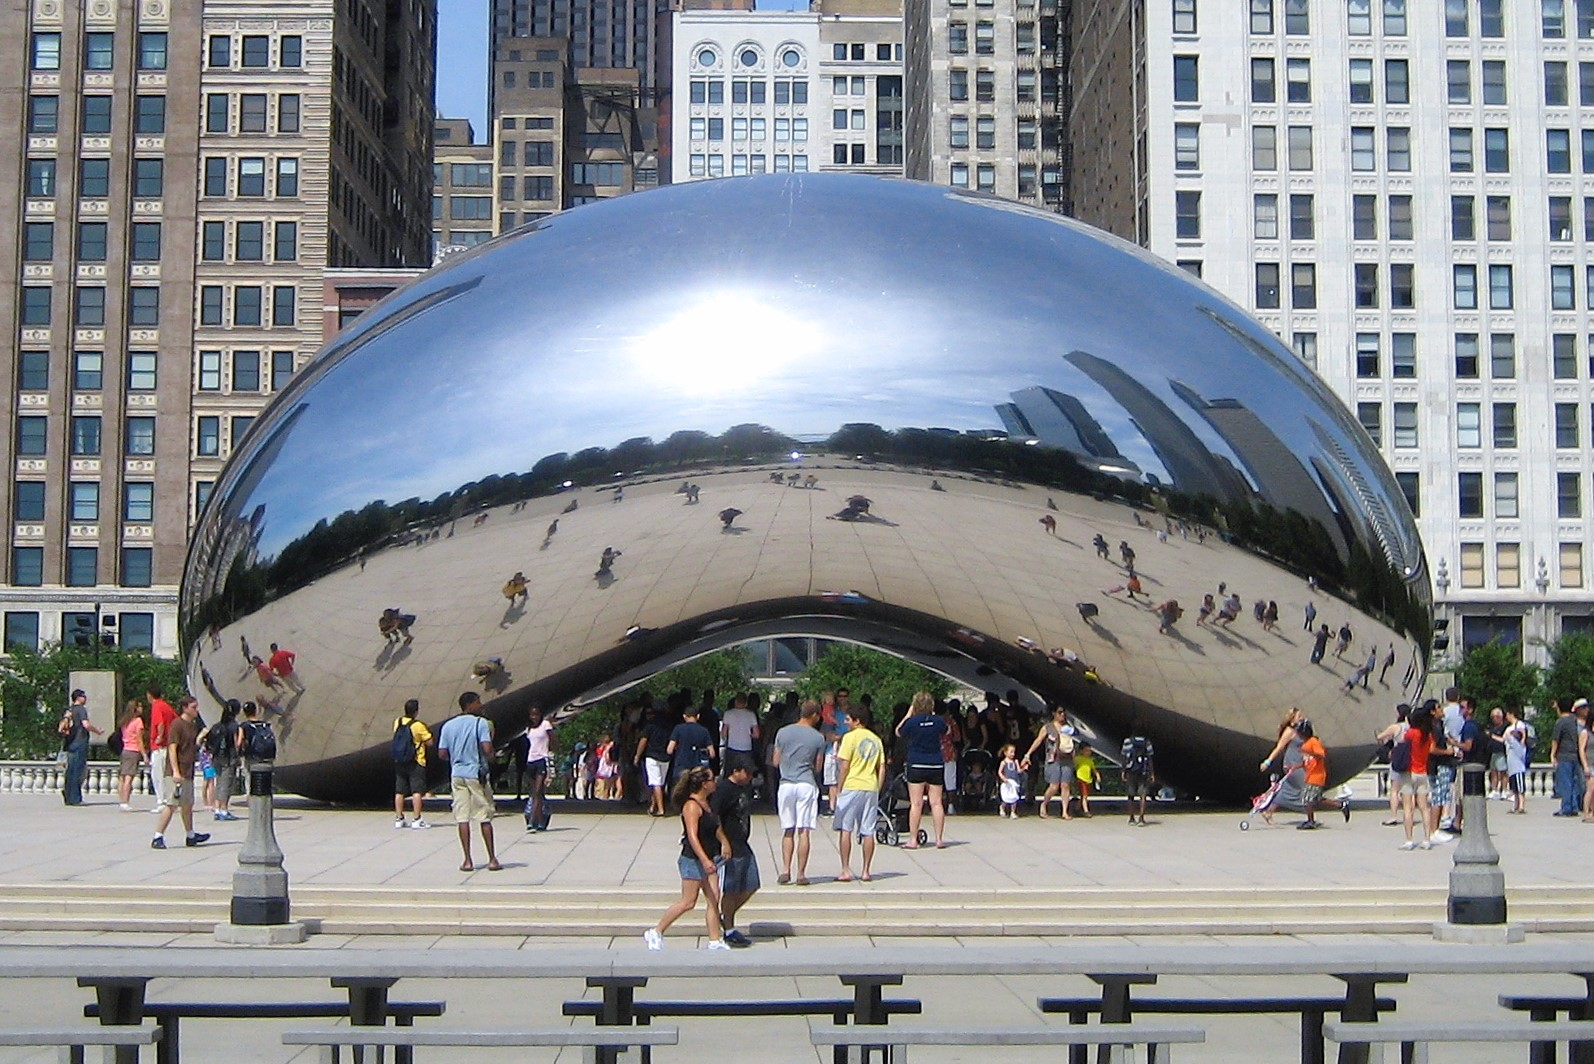
\includegraphics[width=0.55\textwidth]{02_grundlagenDerDeflektometrie/figures/cloud-gate-chicago}
	\caption[Cloud Gate Chicaog - The Bean]{Cloud Gate Chicago - The Bean \cite{cloudGateChicago}}
	\label{img:cloudGateChicago}
\end{figure}

\noindent
In Abbildung \ref{img:cloudGateChicago} erkennt man eine spiegelnde Skulptur, dessen Oberfläche ausschließlich durch die Umgebung und die Spiegelung definiert ist.
Für das menschliche Gehirn ist es zunächst nicht schwierig, die Oberflächenform zu interpretieren.
Das liegt an der Einbeziehung von Kontextinformationen.
So erkennt man z. B. über den Hintergrund und die Umgebung die Form der Skulptur.
Zusätzlich mit der Spiegelung der Szene kann man die Krümmung der Oberfläche deuten.
Wenn man den Hintergrund ausblendet, erkennt man die Schwierigkeit der Thematik (siehe Abbildung \ref{img:cloudGateMitAusschnitt}).

\begin{figure}[H]
	\centering
	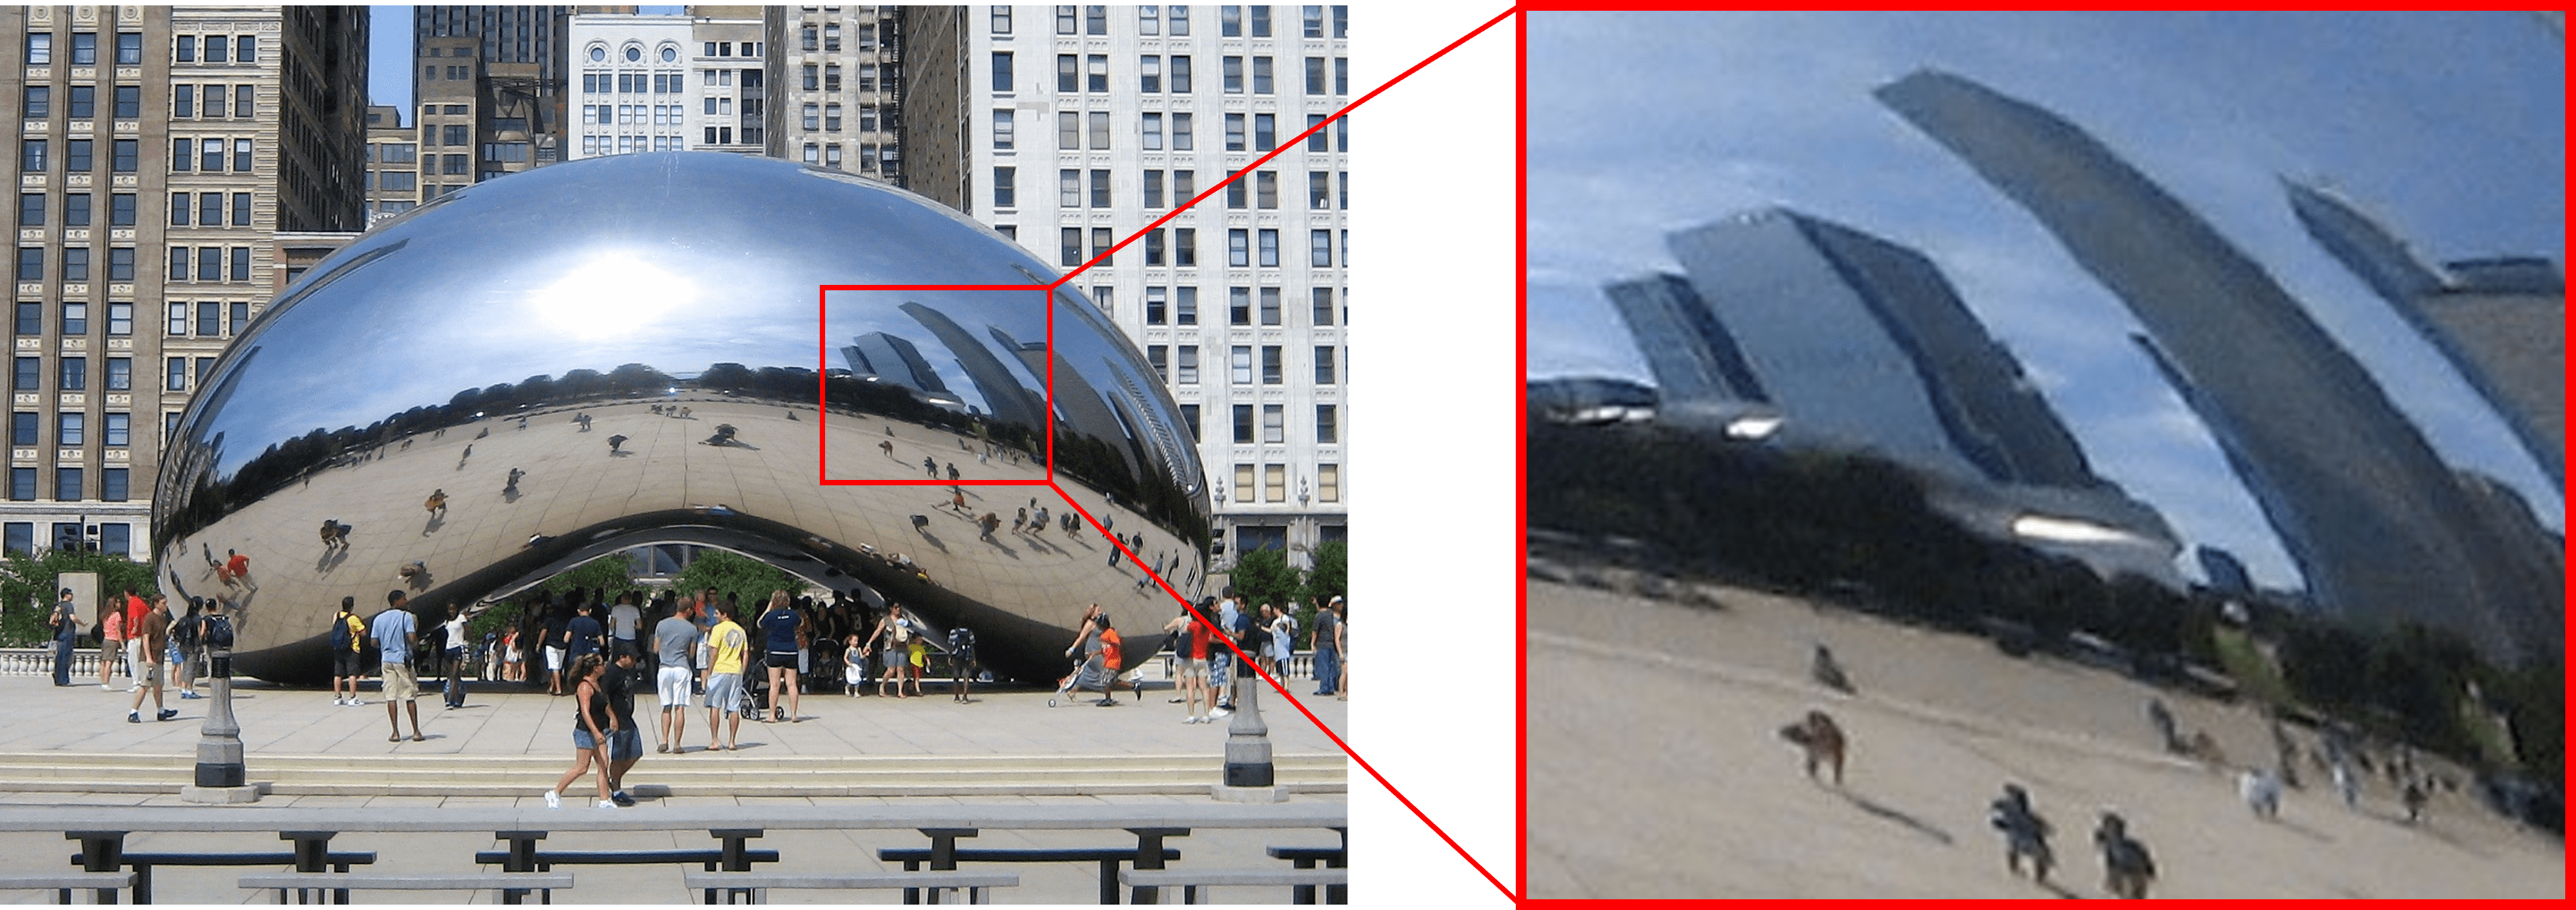
\includegraphics[width=\textwidth]{02_grundlagenDerDeflektometrie/figures/cloudGateMitAusschnitt}
	\caption[Cloud Gate mit Ausschnitt]{Cloud Gate mit Ausschnitt. \textit{in Anlehnung an} \cite{cloudGateChicago}}
	\label{img:cloudGateMitAusschnitt}
\end{figure}

\noindent
Alleine aus dem rechten Ausschnitt von Abbildung \ref{img:cloudGateMitAusschnitt} ist es schon schwieriger zu beurteilen, wie die Skulptur geformt sein könnte.
Zieht man nun Vorwissen über die gespiegelte Szene hinzu, wie z. B. das Wissen über senkrecht stehende Gebäude in Chicago, kann man Aussagen zur Gestalt der lokalen Oberfläche treffen.
Die Schwierigkeit für die automatische Auswertung ist dabei, eine eindeutige Zuordnung zwischen der Szene und dem Spiegelbild aufzustellen.
Diese und ähnliche Aufgaben, in denen Spiegelbilder analysiert werden, fallen in das Themengebiet der Deflektometrie.

\p
Die Definition \ref{def:deflektometrie} öffnet ein großes Feld für verschiedene Verfahren und Anwendungen.
Die Verfahren der Deflektometrie sind auch heute noch Themen für viele Forschungsarbeiten.

%Spiegelnde Oberflächen
{
	\FloatBarrier
    \section{Spiegelnde Oberflächen}
    \label{sec:spiegelndeOberflaechen}
    Zunächst soll auf die zu analysierenden Oberflächen genauer eingegangen werden.
Die deflektometrischen Verfahren werden explizit für spiegelnde Oberflächen entwickelt.
Doch aus welchem Grund trifft man die Unterscheidung zwischen spiegelnden und nicht-spiegelnden Objekten?
Warum lassen sich Verfahren für diffus reflektierende Oberflächen nicht auch für spiegelnden Oberflächen anwenden?
Zur Beantwortung dieser Fragen sollte man die Eigenschaften der Oberflächen genauer betrachten.
Eine diffus reflektierende Oberfläche strahlt die auftreffenden Lichtstrahlen in viele Richtungen ab, wohingegen spekular reflektierende Oberflächen die Lichtstrahlen in eine Richtung reflektieren.
Diffus reflektierende Oberflächen werden als matt oder rau bezeichnet, weil die Lichtstrahlen auf mikroskopischer Ebene auf eine raue Oberfläche treffen.
Spekular reflektierende Oberflächen werden als spiegelnd oder glatt bezeichnet, weil die Lichtstrahlen auf mikroskopischer Ebene auf eine glatte Oberfläche treffen.
Abbildung \ref{tikz:abbGlattUndRau} zeigt diesen Zusammenhang zwischen der mikroskopischen Oberflächenbeschaffenheit und den daraus folgenden Reflexionseigenschaften.

% Abbildung: Glatte und Raue Oberfläche
{
	\begin{figure}[H]
		\centering
		\begin{adjustbox}{width=\textwidth}
	\begin{tikzpicture}[every node/.style={inner sep=0,outer sep=0}]
	
		\node [anchor=north east] (imgGlatt) at (-0.03\textwidth,0) {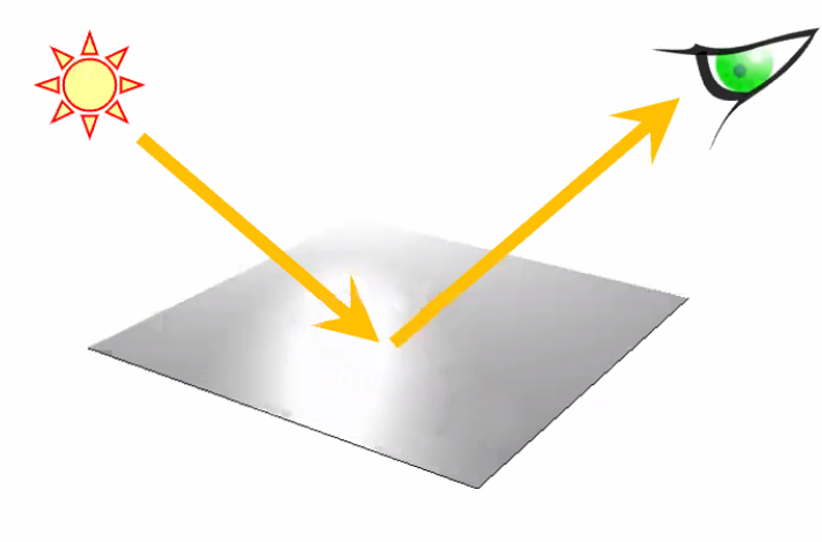
\includegraphics[width=.47\textwidth]{02_grundlagenDerDeflektometrie/spiegelndeOberflaechen/figures/spiegelnd}};
		\node [below=0.2cm of imgGlatt, align=center] {Spiegelnde Oberfläche mit glatter \\ Oberflächenbeschaffenheit};
		\node [anchor=north west] (imgRau) at (0.03\textwidth,0) {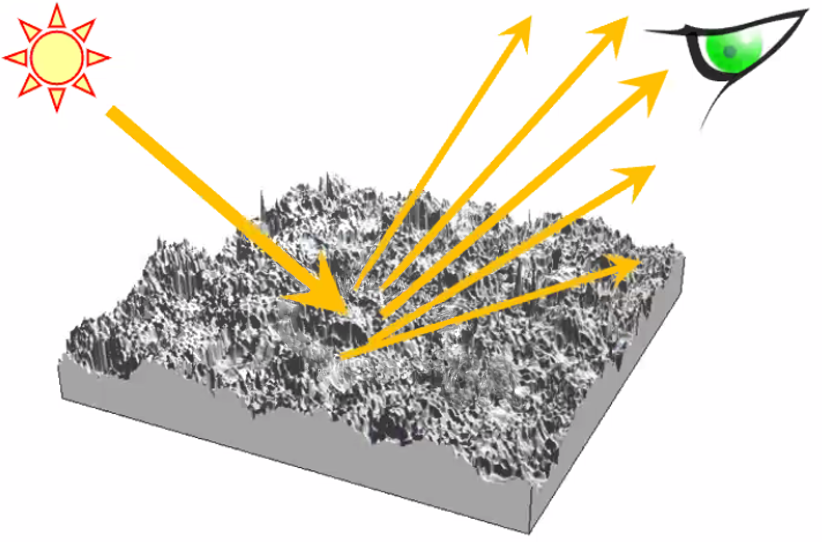
\includegraphics[width=.47\textwidth]{02_grundlagenDerDeflektometrie/spiegelndeOberflaechen/figures/rau}};
		\node [below=0.2cm of imgRau, align=center] {Matte Oberfläche mit rauer \\ Oberflächenbeschaffenheit};
		
	\end{tikzpicture}
\end{adjustbox}
\caption[Spiegelnde und matte Oberflächen]{Spiegelnde bzw. glatte und matte bzw. raue Oberflächen in ihrer mikroskopischen Oberflächenbeschaffenheit. \cite{jenaerOK}}
		\label{tikz:abbGlattUndRau}
	\end{figure}
}
%
\noindent
Durch diese unterschiedliche Reflexionsarten eignen sich für die Oberflächen unterschiedliche Szenen zur Auswertung der Krümmung.
Während spiegelnde Oberfläche ein abbildendes System der Szene darstellt, lässt sich eine Szene über die matte Oberfläche nicht durch eine Spiegelung beobachten.
Für matte Oberflächen eignet sich daher eine Projektion mit viel Licht zur Beobachtung einer Szene.
Für spiegelnde Oberflächen ist dies aufgrund der hohen Reflektivität ungeeignet, stattdessen verwendet man zur Darstellung einer Szene direkt einen Bildschirm (siehe Abbildung  \ref{tikz:abbDeflektometrieVSProjektion}).

% Abbildung: Glatte und Raue Oberfläche
{
	\begin{figure}[H]
		\centering
		\begin{adjustbox}{width=\textwidth}
	\begin{tikzpicture}[every node/.style={inner sep=0,outer sep=0}]
	
		\node [anchor=north east] (imgDeflektometrie) at (-0.03\textwidth,0) {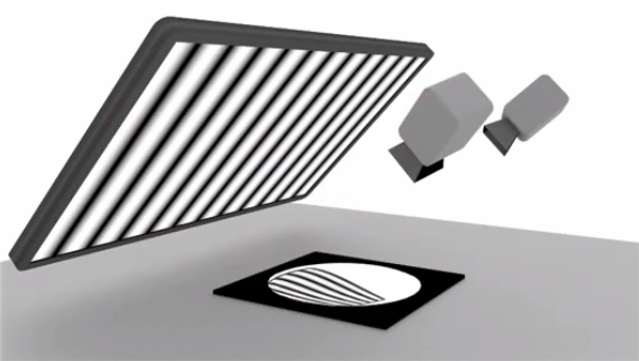
\includegraphics[width=.47\textwidth]{02_grundlagenDerDeflektometrie/spiegelndeOberflaechen/figures/deflektometrie}};
		\node [below=0.2cm of imgDeflektometrie, align=center] {Deflektometrische Verfahren für \\ spiegelnde Oberflächen};
		\node [anchor=north west] (imgProjektion) at (0.03\textwidth,0) {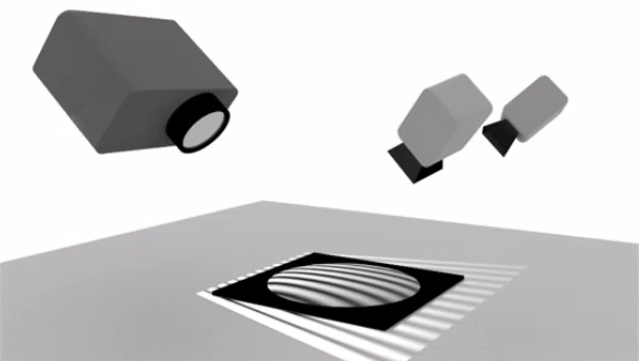
\includegraphics[width=.47\textwidth]{02_grundlagenDerDeflektometrie/spiegelndeOberflaechen/figures/streifenlichtprojektion}};
		\node [below=0.2cm of imgProjektion, align=center] {Streifenlichtprojektion für \\ matte Oberflächen};
		
	\end{tikzpicture}
\end{adjustbox}
\caption[Spiegelnde und matte Oberflächen]{Spiegelnde bzw. glatte und matte bzw. raue Oberflächen in ihrer mikroskopischen Oberflächenbeschaffenheit. \cite{jenaerOK}}
		\label{tikz:abbDeflektometrieVSProjektion}
	\end{figure}
}

\noindent
Im Vergleich erreichen beide Beleuchtungen die Aufnahme einer Szene über der Oberfläche.
Dies ist notwendig um bestimmte Aussagen über die Prüfobjekte treffen zu können.
Der wesentliche Unterschied der beiden Verfahren besteht in der Messempfindlichkeit.
Die deflektometrischen Messverfahren sind neigungssensitiv, da die Reflexion direkt von der Oberflächennormale an den auftreffenden Stellen abhängt.
Im Gegensatz dazu ist die Streifenlichtprojektion durch das Hinzufügen einer Projektionslinse ein höhensensitives Messverfahren für diffus reflektierende Objekte.
Die Oberflächenneigung selbst beeinflusst die aufgenommene Szene bei der Streifenlichtprojektion nicht sehr stark.
Durch die unterschiedliche Funktionsweise der Beleuchtungen für spiegelnde und matte Oberflächen verwendet auch unterschiedliche Verfahren zur Auswertung der Messungen.
Dennoch behandelt man eine ähnliche Fragestellung und findet somit auch Analogien in den Verfahren.

\p
Zuletzt ist es noch wichtig die Besonderheiten von transparenten Objekten zu untersuchen.
Die Oberflächen klarer transparenter Objekte sind glatt und gehören somit zur Kategorie der spiegelnden Oberflächen.
Entscheidend für die transparente Eigenschaft ist die hohe Lichttransmission solcher Objekte, d. h. die Eigenschaft das eintreffende Licht durch das Objekt durchzulassen.
Das bedeutet, dass das Licht in das Objekt eindringen und innerhalb des Objekts gebrochen und reflektiert werden kann (siehe Abbildung \ref{img:rueckseitenreflex}).

% Abbildung: Rückseitenreflex
\begin{figure}[H]
	\centering
	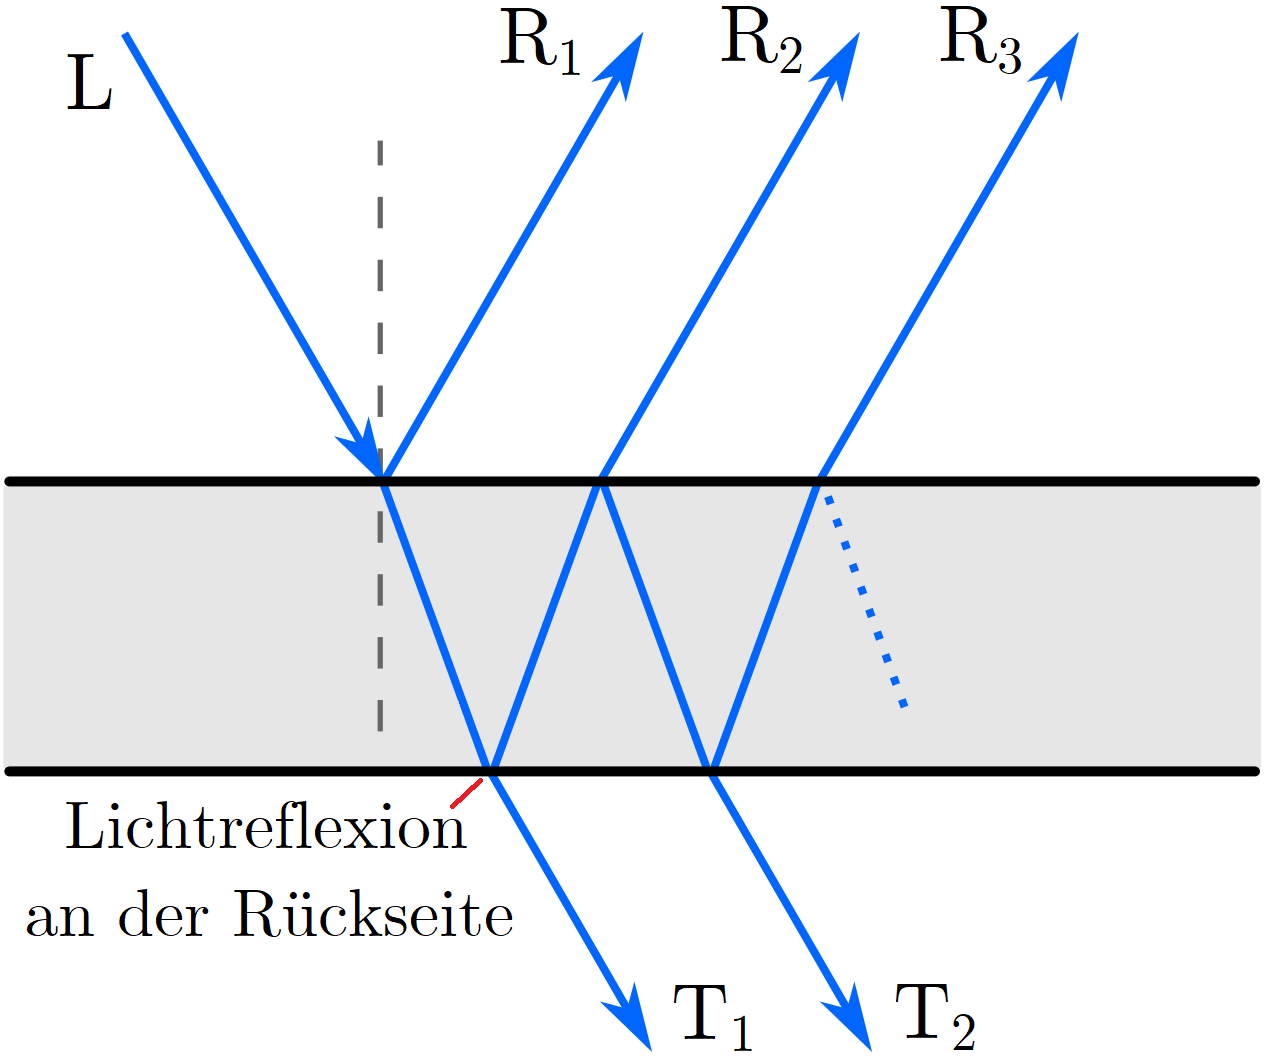
\includegraphics[width=0.4\textwidth]{02_grundlagenDerDeflektometrie/spiegelndeOberflaechen/figures/rueckseitenreflex}
	\caption[Rückseitenreflex]{Brechung und Reflexion an einem ebenen transparenten Objekt. $L$ bezeichnet den eingehenden Lichtstrahl, $R_i$ die reflektierten Lichtstrahlen und $T_i$ die transmittierten Lichtstrahlen. \cite{deflektometrieScheiben}}
	\label{img:rueckseitenreflex}
\end{figure}

\noindent
Die Lichtreflexion an der Rückseite des Objekts wird Rückseitenreflex genannt.
Dadurch entsteht im Sichtfeld eine Über\-la\-ge\-rung von einer doppelt reflektierten Szene.
Diese Über\-la\-ge\-rung sorgt für Probleme in der Auswertung der aufgenommenen Bildern.
In Abbildung \ref{img:rueckseitenreflexBeispiel} wird der Rückseitenreflex einer Glaslinse dargestellt.
Die Szene ist dabei eine Streifenbeleuchtung durch einen Bildschirm.

% Abbildung: Rückseitenreflex Beispiel
\begin{figure}[H]
	\centering
	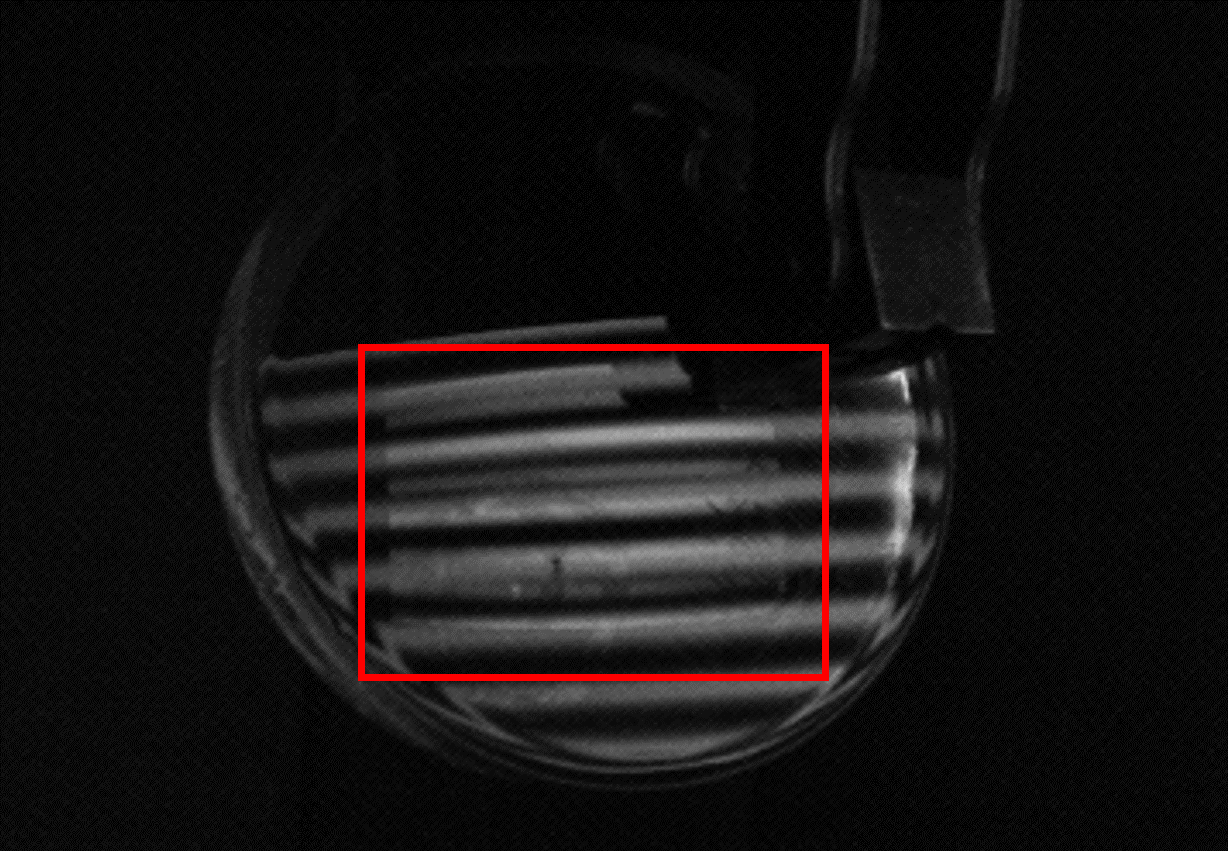
\includegraphics[width=0.5\textwidth]{02_grundlagenDerDeflektometrie/spiegelndeOberflaechen/figures/rueckseitenreflexBeispiel}
	\caption[Beispiel Rückseitenreflex]{Beispiel eines Rückseitenreflex einer transparenten Glaslinse. Im roten Rechteck erkennt man eine leichte zweite Reflexion.}
	\label{img:rueckseitenreflexBeispiel}
\end{figure}

\noindent
Den Effekt des Rückseitenreflex lässt sich durch bestimmte Verfahren, wie z. B. eine undurchsichtige Beschichtung der Oberfläche des transparenten Objekts vermeiden.
Dadurch beschädigt man aber auch die Oberfläche des untersuchten Objekts.
Andere Mög\-lich\-keiten dies zu reduzieren sind spezielle Beleuchtungen, z. B. statt LCD-Bildschirme kann man Beleuchtungen mit Lichtwellen im ultravioletten Bereich verwenden \cite{invisionUVDeflektometrie}.
Ganz umgehen kann man den Rückseitenreflex indem man keine Reflexion aufnimmt, sondern mit Durchlicht arbeitet.
Damit kommen man allerdings auch Einschränkungen einher, die bestimmte Verfahren ausschließen.

\p
Mit diesem Wissen über den Einsatz von bestimmter Beleuchtungsstrategien für spezielle Oberflächen und Objekte, kann man Verfahren beschreiben zur Analyse von spiegelnden Oberflächen.
}

%Rekonstruktion von spiegelnden Oberflächen
{
	\FloatBarrier
    \section{Rekonstruktion von spiegelnden Oberflächen}
    \label{sec:rekonstruktion}
    Das Hauptforschungsgebiet der gegenwärtigen Deflektometrie ist die Generierung von dreidimensionalen Modellen von spiegelnden Objektoberflächen.
Der Aufbau eines solchen Anwendungsfalls sieht eine Beleuchtungseinheit (z. B. einen Bildschirm), einen Sensor (z. B. eine Kamera) und ein zu untersuchendes Objekt vor.

\begin{figure}[H]
	\centering
	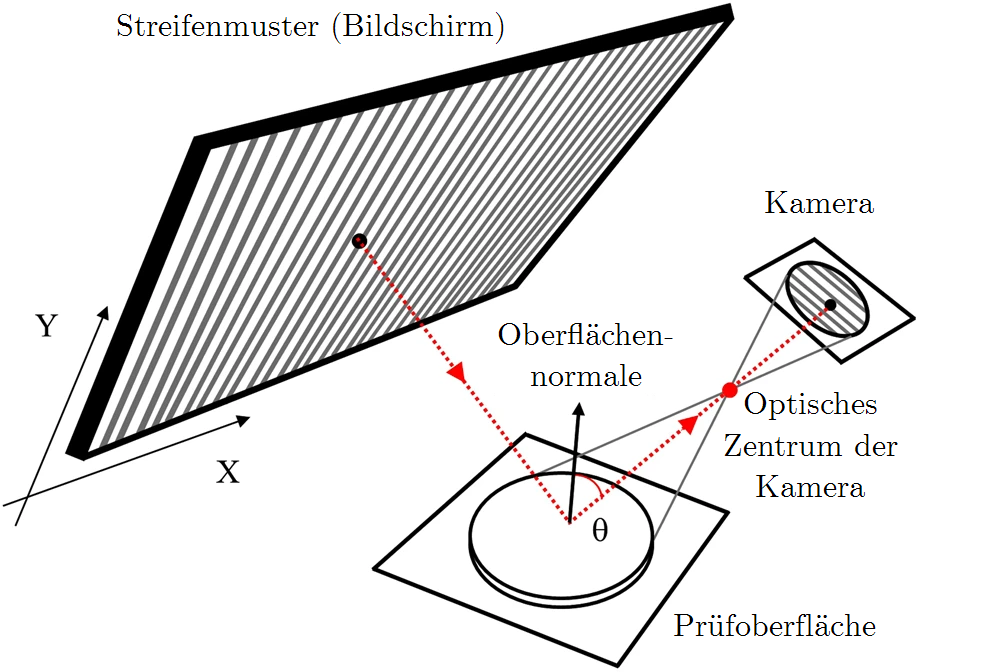
\includegraphics[width=0.7\textwidth]{02_grundlagenDerDeflektometrie/rekonstruktion/figures/nature-articel-nr1}
	\caption[Aufbau einer Deflektometrie-Prüfstation]{Aufbau einer Deflektometrie-Prüfstation. \textit{in Anlehnung an} \cite{aufbau}}
	\label{img:aufbau}
\end{figure}

\noindent
Wie in Abbildung \ref{img:aufbau} angedeutet, wird ein Muster als bekannte Szene auf ein Prüfobjekt abgebildet und anschließend von einer Kamera aufgenommen.
Das grundlegende Prinzip basiert darauf, dass jeder durch die Kamera aufgenommene Punkt des Objekts dem Punkt auf dem Bildschirm zugeordnet wird, der den Objektpunkt beleuchtet bzw. der am Objektpunkt in die Kamera reflektiert wird.
Dabei ordnet man jedem Pixel des projizierten Musters sein zugehöriges Pixel des erzeugten Musters auf dem Bildschirm zu.
Durch diese Zuordnung von Kamera- und Bildschirmpunkten lassen sich Neigungsinformationen der Oberfläche berechnen.
Dies kann durch Strahlenverfolgungen erreicht werden.
In Abbildung \ref{img:aufbau} lässt sich das über die in Rot eingezeichneten Vektoren erkennen.
Die Schwierigkeit liegt in der eindeutigen Zuordnung zwischen der Szene und dem Spiegelbild.
Hierfür gibt es verschiedene Ansätze, dies zu erreichen.
Grundlegend ist dabei die Kodierung der Objektoberfläche (siehe Definition \ref{def:kodierungOberflaeche}), damit diese durch die Kamera aufgenommen werden kann.
Die Kamera digitalisiert dann die kodierte Oberfläche zu einem oder mehreren Bildern.
Unter Berücksichtigung der Kodierung können die Bilder durch einen entsprechenden Softwarealgorithmus dekodiert werden und man erhält damit die Zuordnung zwischen der Szene und dem Spiegelbild (siehe Abbildung \ref{tikz:abbKodierungUndDekodierung}).
%
% Definition: Kodierung der Objektoberfläche
\begin{Definition}{Kodierung der Objektoberfläche}{def:kodierungOberflaeche}
	Die Abbildung einer oder mehrerer vordefinierter Szenen auf eine spiegelnde Oberfläche wird als \textit{Kodierung der Objektoberfläche} bezeichnet.
	Das Ziel ist es dabei die Punkte aus der Szene eindeutig durch eine oder mehrere Aufnahmen der Oberfläche zu identifizieren.
\end{Definition}
%
%
% Abbildung: Kodierung und Dekodierung
{
	\begin{figure}[H]
		\centering
		\begin{adjustbox}{width=\textwidth}
	\begin{tikzpicture}
	[
		rectnode/.style={rectangle, draw=red!60, fill=red!5, very thick, minimum width={3cm}, font=\small, rounded corners},
		ellipsenode/.style={ellipse, draw=green!60, fill=green!5, very thick, minimum width={3cm}, font=\small},
		calloutnode/.style={rectangle callout, draw=RoyalPurple, fill=RoyalPurple!5, text=RoyalPurple, font=\footnotesize, rounded corners},
	]

		\node[ellipsenode] (source) {Quelle};
		\node[rectnode] (encoder) [right=of source] {Kodierung};
		\node[rectnode] (channel) [below right=of encoder] {Digitalisierung};
		\node[rectnode] (decoder) [below left=of channel] {Dekodierung};
		\node[ellipsenode] (drain) [left=of decoder]{Ergebnis};		
		
		\draw[->] (source.east) -- (encoder.west);
		\draw[->] (encoder.east) -| (channel.north);
		\draw[->] (channel.south) |- (decoder.east);
		\draw[->] (decoder.west) -- (drain.east);
		
		\node[right=of channel, font=\small, align=center] (noise) {Rauschen,\\ Unschärfe};
		\draw[->] (noise.west) -- (channel.east);
		
		\node[calloutnode] (surface) [callout absolute pointer=(source.north), above=of source.east, anchor=east] {Objektoberfläche};
		\node[calloutnode] (illumination) [callout absolute pointer=(encoder.north), above=of encoder.east, anchor=east] {Beleuchtung};
		\node[calloutnode] (camera) [callout absolute pointer=(channel.30), above=of channel.east, anchor=east] {Kamera};
		\node[calloutnode] (software) [callout absolute pointer=(decoder.north), above=of decoder.east, anchor=east] {Algorithmus};
		\node[calloutnode] (result) [callout absolute pointer=(drain.north), above=of drain.east, anchor=east] {Zuordnung};
		
	\end{tikzpicture}
\end{adjustbox}
\caption[Kodierung und Dekodierung der Objektoberfläche]{Kodierung und Dekodierung der Objektoberfläche.}
		\label{tikz:abbKodierungUndDekodierung}
	\end{figure}
}

\noindent
Die Art, wie man die Informationen in den digitalen Kanal überträgt, ist entscheidend für eine gute Zuordnung.
Aus dem Grund werden sich in wissenschaftlichen Forschungsarbeiten einige Gedanken über die Kodierung der Objektoberfläche gemacht.
Auf eine Auswahl von Möglichkeiten aus dem heutigen wissenschaftlichen Stand soll im Folgenden eingegangen werden.
%
% Phasenkodierung
{
	\FloatBarrier
    \subsection{Phasenkodierung}
    \label{sub:phasenKodierung}
    Die am häufigsten eingesetzte Kodiermethode im Kontext der Deflektometrie ist die Phasenkodierung.
Dieser Ansatz wird im Themengebiet der \glqq Phasenmessenden Deflektometrie\grqq ~beschrieben.
Dabei verwendet man Streifenmuster die entlang der Ausbreitung der Streifen, den Grauwertverlauf einer trigonometrischen Funktion (z. B. Sinus- oder Kosinus-Funktion) annehmen.
Solche Muster nennt man auch sinusoidale Streifenmuster.
Die Szene bzw. der Monitor wird dabei über die Phase der Sinus-Funktion kodiert.
Das heißt, jeder Punkt auf einem Monitor, angegeben durch eine $x$- und eine $y$-Koordinate, wird durch eine Phase $\phi_x$ in $x$-Richtung und eine Phase $\phi_y$ in $y$-Richtung kodiert.
Verwendet man Streifenmuster, stellt man die Kodierung in zwei Bildern dar.
Das erste Bild kodiert die Spaltenpositionen durch die Phasen $\phi_x$ und das zweite Bild kodiert die Zeilenpositionen durch die Phasen $\phi_y$ (siehe Abbildung \ref{tikz:abbSinusoidaleStreifenmuster}).

\begin{figure}[H]
	\centering
		\begin{adjustbox}{width=\textwidth}
	\begin{tikzpicture}[every node/.style={inner sep=0,outer sep=0}]
	
		\node [anchor=north east] (imgSpalten) at (-0.03\textwidth,0) {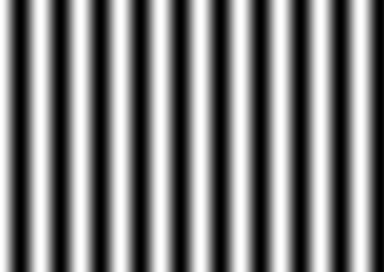
\includegraphics[frame,width=.47\textwidth]{02_grundlagenDerDeflektometrie/rekonstruktion/phasenKodierung/figures/sinusoidalesXMuster}};
		\node [below=0.2cm of imgSpalten, align = center] {Sinusoidales Muster zur Kodierung \\ der Spalten durch die Phasen $\phi_x$};
		\node [anchor=north west] (imgZeilen) at (0.03\textwidth,0) {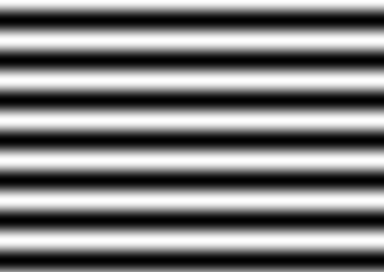
\includegraphics[frame,width=.47\textwidth]{02_grundlagenDerDeflektometrie/rekonstruktion/phasenKodierung/figures/sinusoidalesYMuster}};
		\node [below=0.2cm of imgZeilen, align = center] {Sinusoidales Muster zur Kodierung \\ der Zeilen durch die Phasen $\phi_y$};
		
	\end{tikzpicture}
\end{adjustbox}
\caption[Sinusoidale Streifenmuster]{Sinusoidale Streifenmuster zur Kodierung der Szene durch die Phasen $\left(\phi_x,\phi_y\right)$.}
		\label{tikz:abbSinusoidaleStreifenmuster}
\end{figure}

\noindent
Der Vorteil ist dabei die Kodierung durch die Grauwerte, die unabhängig von benachbarten Positionen dekodiert werden können.
Zur Dekodierung müssen aus den Grauwerten zunächst die Phasen bestimmt werden.
Dies funktioniert über ein sogenanntes Phasenschiebeverfahren \cite{carre}, bei dem weitere Bildaufnahmen mit Phasenverschiebungen der trigonometrischen Funktion vorgenommen werden.
Durch die Periodizität der verwendeten trigonometrischen Funktion sind die bestimmten Phasen zunächst noch relativ zu den einzelnen Perioden angegeben.
In einem weiteren Schritt muss eine sogenannte Phasenentfaltung bzw. ein \glqq Phase Unwrap\grqq ~durchgeführt werden (siehe auch Definition \ref{def:phasenentfaltung}), damit die absoluten Phasen $\left(\phi_x,\phi_y\right)$ bestimmt werden können.
Die Dekodierung über das \glqq Phase Unwrap\grqq ~erfolgt dabei durch die Verwendung von weiteren sinusoidalen Streifenmustern mit unterschiedlicher Frequenz.
Diese Art der Kodierung erfordert deshalb weitere Bilder.
Ein solches Verfahren wird im Kapitel \ref{sec:bestimmungDeflektometrischeRegistrierung} genauer beschrieben.

\p
Es sind damit zunächst mehrere Bildaufnahmen erforderlich.
Da solche Verfahren damit mehr Ressourcen verwenden, fokussieren sich einige Forschungsarbeiten darauf, die Anzahl der benötigten Muster zu reduzieren.
Der heutige technische Stand ermöglicht es bereits z. B. durch Überlagerung von Mustern und weiteren Optimierungen, die Phasendekodierung durch eine einzige Kameraaufnahme umzusetzen (vgl. \cite{waveletPMD}).
Allerdings wird dadurch mehr Information kodiert auf gleichem Ort, wodurch Unschärfen und starke Krümmungen des Objekts das Ergebnis der deflektometrischen Messung stärker verfälschen können.
}
%
% Frequenzkodierung
{
	\FloatBarrier
    \subsection{Frequenzkodierung}
    \label{sub:frequenzKodierung}
    Als Alternative zur Phasenkodierung kann man die Sinus-Funktion auch nutzen um die Ortskoordinaten des Bildschirms über Frequenzen zu kodieren.
Hierfür eignet sich die Darstellung der Koordinaten in der Polarform.
%
\begin{equation*}
	\left(x,y\right) \mapsto \left(r,\phi\right)
\end{equation*}
%
Wenn man im Folgenden den Radius $r$ einer speziellen Frequenz und die Phase $\phi$ als Phasenverschiebung einer Sinus-Funktion zuweist, erhält man zeitabhängige Muster.
So könnte zum Beispiel durch
%
\begin{equation*}
	f_t \left(r,\phi\right) = 1 + \sin \left(2 \pi r t + \phi \right)
\end{equation*}
%
die Kodierung der Szene in Abhängigkeit der Zeit $t$ angegeben sein.
In Abbildung \ref{tikz:abbFrequenzkodierteMuster} wird eine Kodierung dieser Art zu bestimmten Zeitpunkten abgebildet.
%
\begin{figure}[H]
	\centering
	\begin{adjustbox}{width=\textwidth}
	\begin{tikzpicture}[every node/.style={inner sep=0,outer sep=0}]
	
		\node [anchor=north east] (freq0) at (-0.03\textwidth,0) {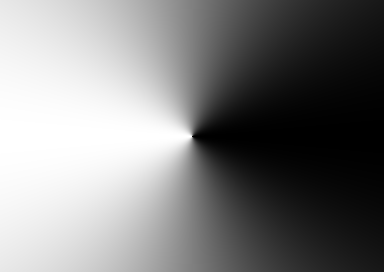
\includegraphics[frame,width=.47\textwidth]{02_grundlagenDerDeflektometrie/rekonstruktion/frequenzKodierung/figures/frequenzKodiertT0}};
		\node [below=0.2cm of freq0] (cap0) {Muster zum Zeitpunkt $t = 0$};
		\node [anchor=north west] (freq1) at (0.03\textwidth,0) {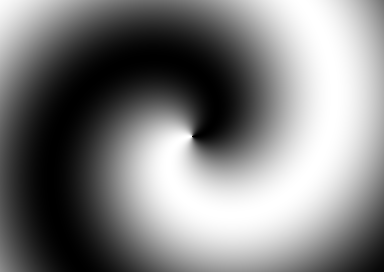
\includegraphics[frame,width=.47\textwidth]{02_grundlagenDerDeflektometrie/rekonstruktion/frequenzKodierung/figures/frequenzKodiertT1}};
		\node [below=0.2cm of freq1] (cap1) {Muster zum Zeitpunkt $t = 1$};
		
		\node [below=1cm of freq0.south east, anchor=north east] (freq4) {
\includegraphics[frame,width=.47\textwidth]{02_grundlagenDerDeflektometrie/rekonstruktion/frequenzKodierung/figures/frequenzKodiertT4}};
		\node [below=0.2cm of freq4] {Muster zum Zeitpunkt $t = 4$};
		\node [below=1cm of freq1.south west, anchor=north west] (freq10) {
\includegraphics[frame,width=.47\textwidth]{02_grundlagenDerDeflektometrie/rekonstruktion/frequenzKodierung/figures/frequenzKodiertT10}};
		\node [below=0.2cm of freq10] {Muster zum Zeitpunkt $t = 10$};
		
	\end{tikzpicture}
\end{adjustbox}
\caption[Muster der Frequenzkodierung]{Muster der Frequenzkodierung der Szene zu festen Zeitpunkten $t$.}
	\label{tikz:abbFrequenzkodierteMuster}
\end{figure}
%
\noindent
Zur Dekodierung muss hier über eine gewisse Zeit die Frequenz der einzelnen Bildpunkte gemessen werden.
Zusätzlich muss der Phasenwinkel bestimmt werden.
Dafür kann ein ähnliches Verfahren wie auch bei der Bestimmung der Phase im vorhergehenden Abschnitt \ref{sub:phasenKodierung} eingesetzt werden.
Zur Optimierung des Rechenaufwands ist es auch möglich, jeder Ortskoordinate eine eigene Frequenz zuzuweisen, damit man sich die Bestimmung der Phase sparen kann.

\p
Da in diesem Kodierverfahren nicht mehr die Grauwerte des Bildes selbst den Ort kodieren, ist es unempfindlich gegenüber Nichtlinearitäten in den Anzeige- oder Aufnahmefarben.
Außerdem lassen sich mehrere Signale überlagern und genau durch die Frequenz trennen.
Ein großer Nachteil im Vergleich zur Phasenkodierung ist allerdings die lange Messzeit der Frequenz \cite{jenaerOK}.
}
%
% Stochastische Kodierung
{
	\FloatBarrier
    \subsection{Stochastische Kodierung}
    \label{sub:stochastischeKodierung}
    Bei der stochastischen Kodierung nutzt man ein zufällig generiertes Muster als Szene.
Geeignet für dieses Verfahren sind sogenannte \glqq Specklemuster\grqq ~\cite{specklePattern}.
Es handelt sich dabei um bandbegrenzte Muster mit zufällig verteilten Grauwerten.
Aufgrund der Unschärfe und des Rauschens in den Bildern, welche durch eine Kameraaufnahme einfließen, ist die Bandbegrenztheit notwendig, um eine Dekodierung zu ermöglichen.
Abbildung \ref{img:speckleMuster} zeigt ein solches Muster.
%
\begin{figure}[H]
	\centering
	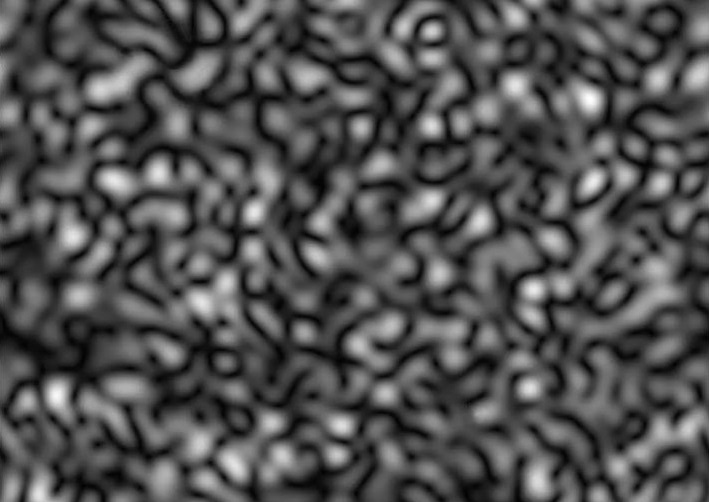
\includegraphics[frame,width=0.5\textwidth]{02_grundlagenDerDeflektometrie/rekonstruktion/stochastischeKodierung/figures/speckleMuster}
	\caption[Specklemuster]{Specklemuster.}
	\label{img:speckleMuster}
\end{figure}
%
\noindent
Das Grundprinzip der Dekodierung für dieses Kodierverfahren ist das Verfolgen der Punkte beim Verschieben des Specklemusters.
Es wird zunächst die Spiegelung des Specklemusters auf der Objektoberfläche aufgenommen und ein Referenzpunkt definiert.
Nach der Verschiebung des Specklemusters (z. B. in x-Richtung) wird dieser Referenzpunkt in dem zweiten Bild über seine Umgebung gesucht.
Dabei verwendet man einen Algorithmus zur Berechnung der zweidimensionalen Bildkorrelation, der die höchste Übereinstimmung mit der Umgebung sucht.
Wenn der verschobene Referenzpunkt gefunden wurde, wird an derselben Stelle der Punkt im ersten Bild markiert.
Der markierte Punkt ist dann der neue Referenzpunkt, der im zweiten Bild gesucht wird.
Dieser Vorgang wiederholt sich, solange die Referenzpunkte im Bild liegen.
Abbildung \ref{img:prinzipStoKodierung} zeigt schematisch das Verfahren zur Dekodierung.
%
\begin{figure}[H]
	\centering
	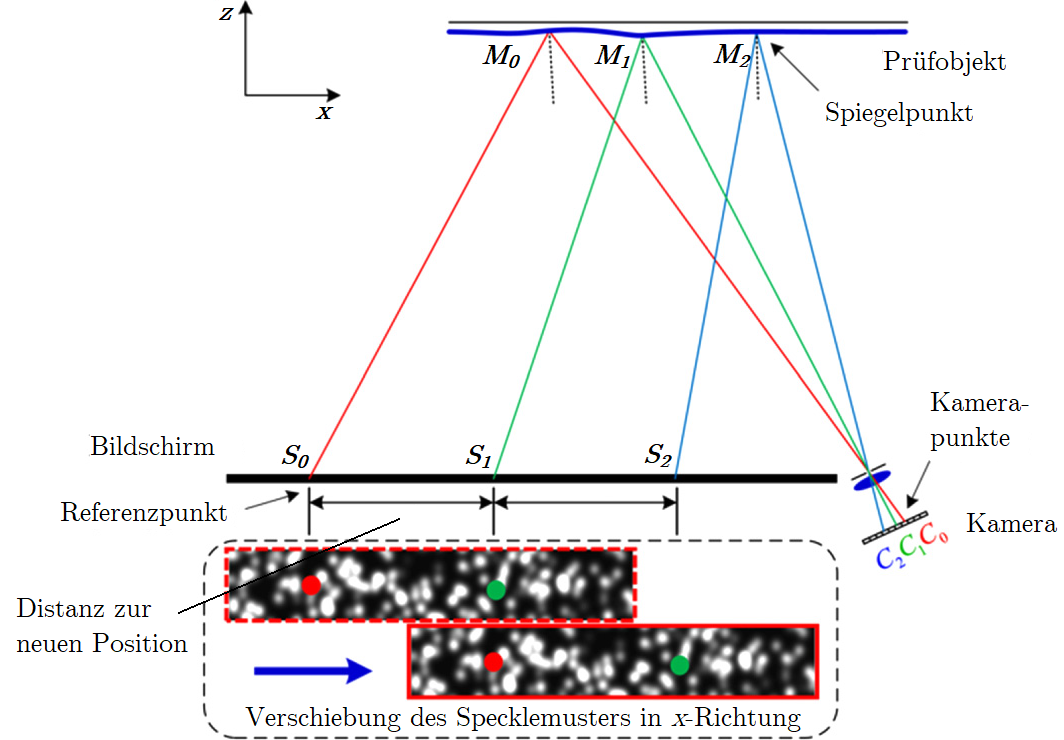
\includegraphics[width=0.9\textwidth]{02_grundlagenDerDeflektometrie/rekonstruktion/stochastischeKodierung/figures/Prinzip}
	\caption[Prinzip der Zuordnung einer stochastischen Kodierung]{Prinzip der Zuordnung einer stochastischen Kodierung. \textit{in Anlehnung an} \cite{specklePattern}}
	\label{img:prinzipStoKodierung}
\end{figure}
%
\noindent
Führt man dasselbe auch für eine andere Richtung (z. B. in y-Richtung) durch, erhält man ein Raster auf dem Objekt, an dem die Objektpunkte zugeordnet wurden (siehe Abbildung \ref{img:ergebnisStoKodierung}).
%
\begin{figure}[H]
	\centering
	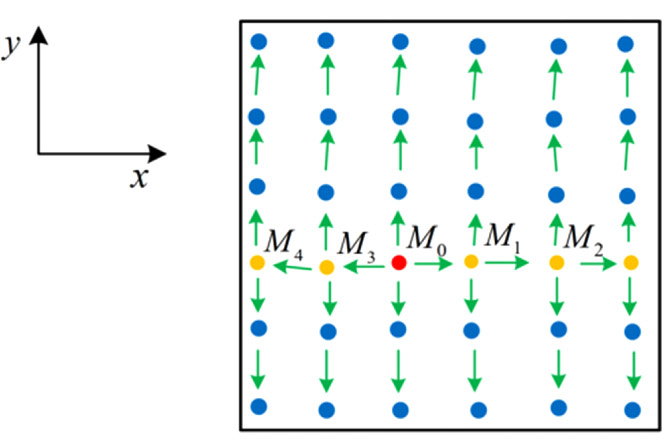
\includegraphics[width=0.4\textwidth]{02_grundlagenDerDeflektometrie/rekonstruktion/stochastischeKodierung/figures/Ergebnis}
	\caption[Ergebnis der Zuordnung einer stochastischen Kodierung]{Ergebnis der Zuordnung einer stochastischen Kodierung. Die grünen Pfeile zeigen an, von welchem Referenzpunkt man auf die nächste Zuordnung kam. \textit{in Anlehnung an} \cite{specklePattern}}
	\label{img:ergebnisStoKodierung}
\end{figure}
%
\noindent
Im Vergleich zu den vorgestellten Kodierverfahren in den vorherigen Abschnitten \ref{sub:phasenKodierung} und \ref{sub:frequenzKodierung} liefert die Dekodierung in diesem Fall nur eine begrenzte Auflösung und keine vollflächige Zuordnung.
Außerdem ist dieses Verfahren nicht anwendbar für Objekte, die eine große Verzerrung des Musters erzeugen, da die zweidimensionalen Bildkorrelation ansonsten die Referenzpunkte nicht finden kann.
Dennoch sind große Vorteile dieses Verfahrens, der geringe Rechenaufwand und die Möglichkeit, durch drei Bilder eine erfolgreiche Dekodierung durchzuführen \cite{specklePattern}.

\p
Im Rahmen der vorliegenden Arbeit wird nicht weiter auf dieses Kodierverfahren eingegangen.
}
%
% Rekonstruktion der Oberfläche und Regularisierungsproblem
{
	\FloatBarrier
    \subsection{Rekonstruktion der Oberfläche und Regularisierungsproblem}
    \label{sub:rekonstruktionUndRegularisierungsproblem}
    Durch das Vorgehen nach Abbildung \ref{tikz:abbKodierungUndDekodierung} und die beschriebenen Kodiermöglichkeiten kann die Zuordnung der Kamerapunkte und der Bildschirmpunkte erfolgen.
Mithilfe weiterer Schritte kann man daraus die Oberfläche rekonstruieren.
%
\begin{figure}[H]
	\centering
	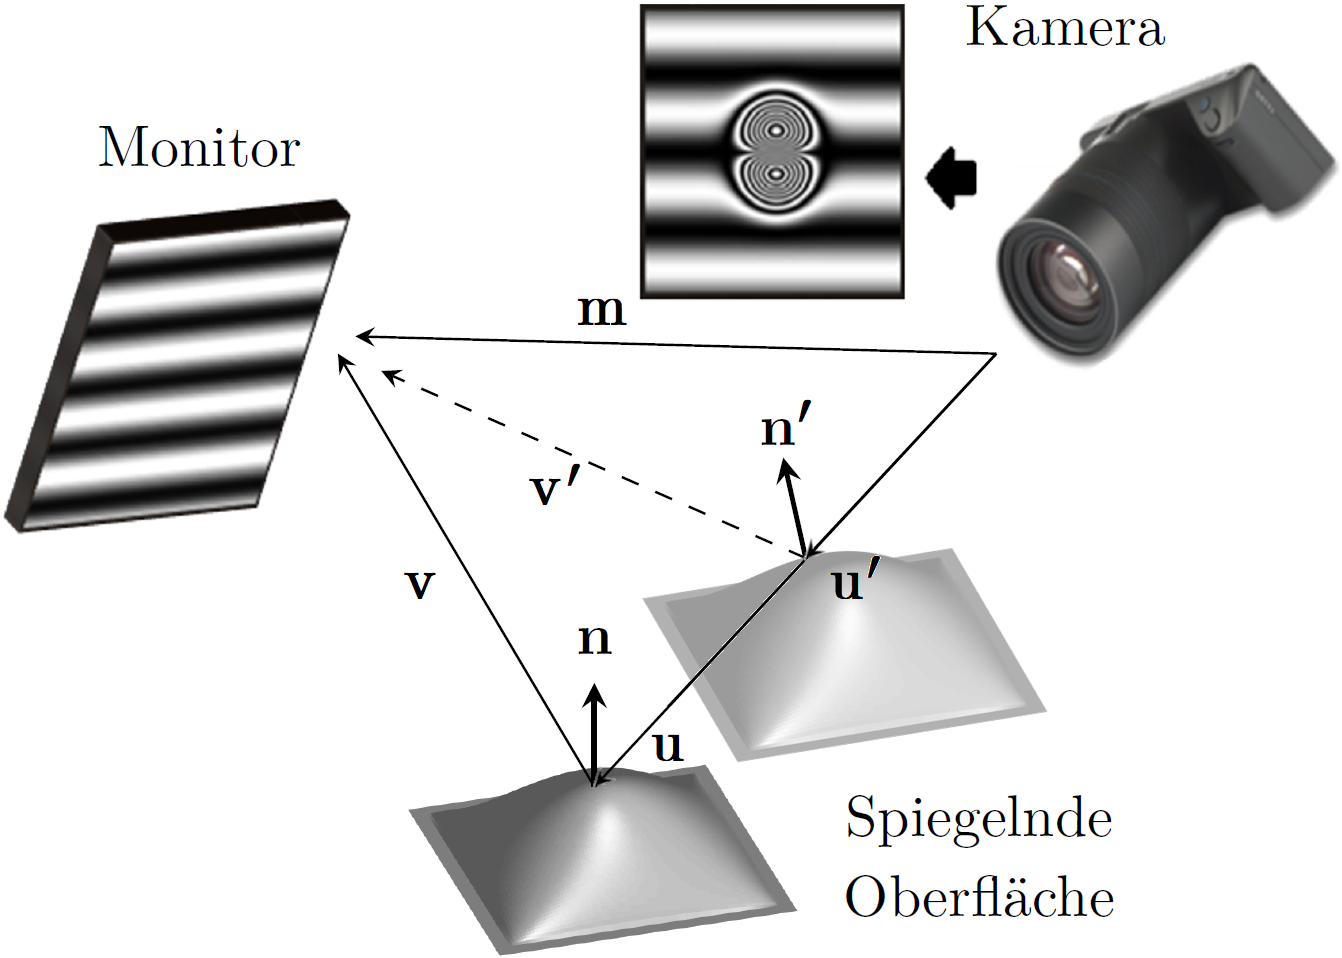
\includegraphics[width=0.7\textwidth]{02_grundlagenDerDeflektometrie/rekonstruktion/rekonstruktionUndRegularisierungsproblem/figures/regularisierungsproblem}
	\caption[Regularisierungsproblem]{Mehrere Positionsmöglichkeiten für die spiegelnde Oberfläche bei selber Zuordnung von Kamera- und Bildschirmpunkten, auch Regularisierungsproblem genannt. \textit{in Anlehnung an} \cite{stereoDeflektometrie}}
	\label{img:regularisierungsproblem}
\end{figure}
%
\noindent
Abbildung \ref{img:regularisierungsproblem} zeigt die Strahlenverfolgung zur Bestimmung der Oberflächennormalen $n$.
Zunächst benötigt man neben der Zuordnung zusätzliche Informationen über den Systemaufbau.
Das umfasst die Positionen und Ausrichtungen der Kamera und des Monitors im Raum, womit man die Zuordnung in Weltkoordinaten angeben kann.
Dadurch ist der Vektor $m$ sowie die Richtung des Sichtvektors $u$ bestimmt.
Es ist zwar bekannt, welcher Kamerapunkt durch welchen Punkt des Bildschirms beleuchtet wird, allerdings ist dadurch das optische System nicht ausreichend beschrieben, um die Länge des Sichtvektors $u$ anzugeben.
Es fehlt die Lage der Oberfläche.
Wäre diese bekannt, könnte der Reflexionsvektor $v$ mit 
\begin{equation*}
	v = m - u
\end{equation*}
bestimmt werden.
Mithilfe des Reflexionsgesetzes kann man aus dem Reflexionsvektor $v$ und dem Sichtvektor $u$ den Normalenvektor $n$ bestimmen:
%
\begin{equation}
	n = \dfrac{v - u}{\left\Vert v - u \right\Vert}
\end{equation}
%
Der Sichtvektor $u$ lässt sich für jeden Kamerapunkt aufstellen.
Berechnet man nach der Überlegung die Normalenvektoren $n$ für jeden Kamerapunkt, erhält man ein Vektorfeld, welches Normalenfeld genannt wird.
Damit wären die Neigungsinformationen der Oberfläche bekannt.

\p
Durch die unzureichende Information über die Lage der spiegelnden Oberfläche, erhält man entlang der Richtung eines Sichtvektors $u$ unendlich viele potenzielle Normalenvektoren $n'$.
Man bekommt somit auch viele verschiedene Normalenfelder für eine eindeutige Zuordnung von Kamera- und Bildschirmpunkten.
Diese Mehrdeutigkeit wird als Regularisierungs- oder Deflektometrieproblem bezeichnet.
Zur Auflösung des Regularisierungsproblems gibt es verschiedene Ansätze.
Ein solcher Ansatz ist die Stereo-Methode.
Dabei werden zwei Aufnahmen aus unterschiedlichen Positionen verwendet.
Man bestimmt für beide Aufnahmen jeweils eine Zuordnung von Kamera- und Bildschirmpunkten.
Somit entstehen für beiden Aufnahmen mehrere potenzielle Normalenfelder.
Bestimmt man die Korrelation zwischen den Normalenfeldern der unterschiedlichen Aufnahmen, sollte man eine Lage finden, an denen die Normalenfelder übereinstimmen.
Das Normalenfeld in dieser Lage entspricht damit dem tatsächlichen Normalenfeld (siehe Abbildung \ref{img:stereoVerfahren}).
Dieses und auch weitere Verfahren zur Auflösung des Regularisierungsproblems wird in der Dissertation von J. Balzer näher thematisiert\cite{regularisierungsproblem}.
%
\begin{figure}[H]
	\centering
	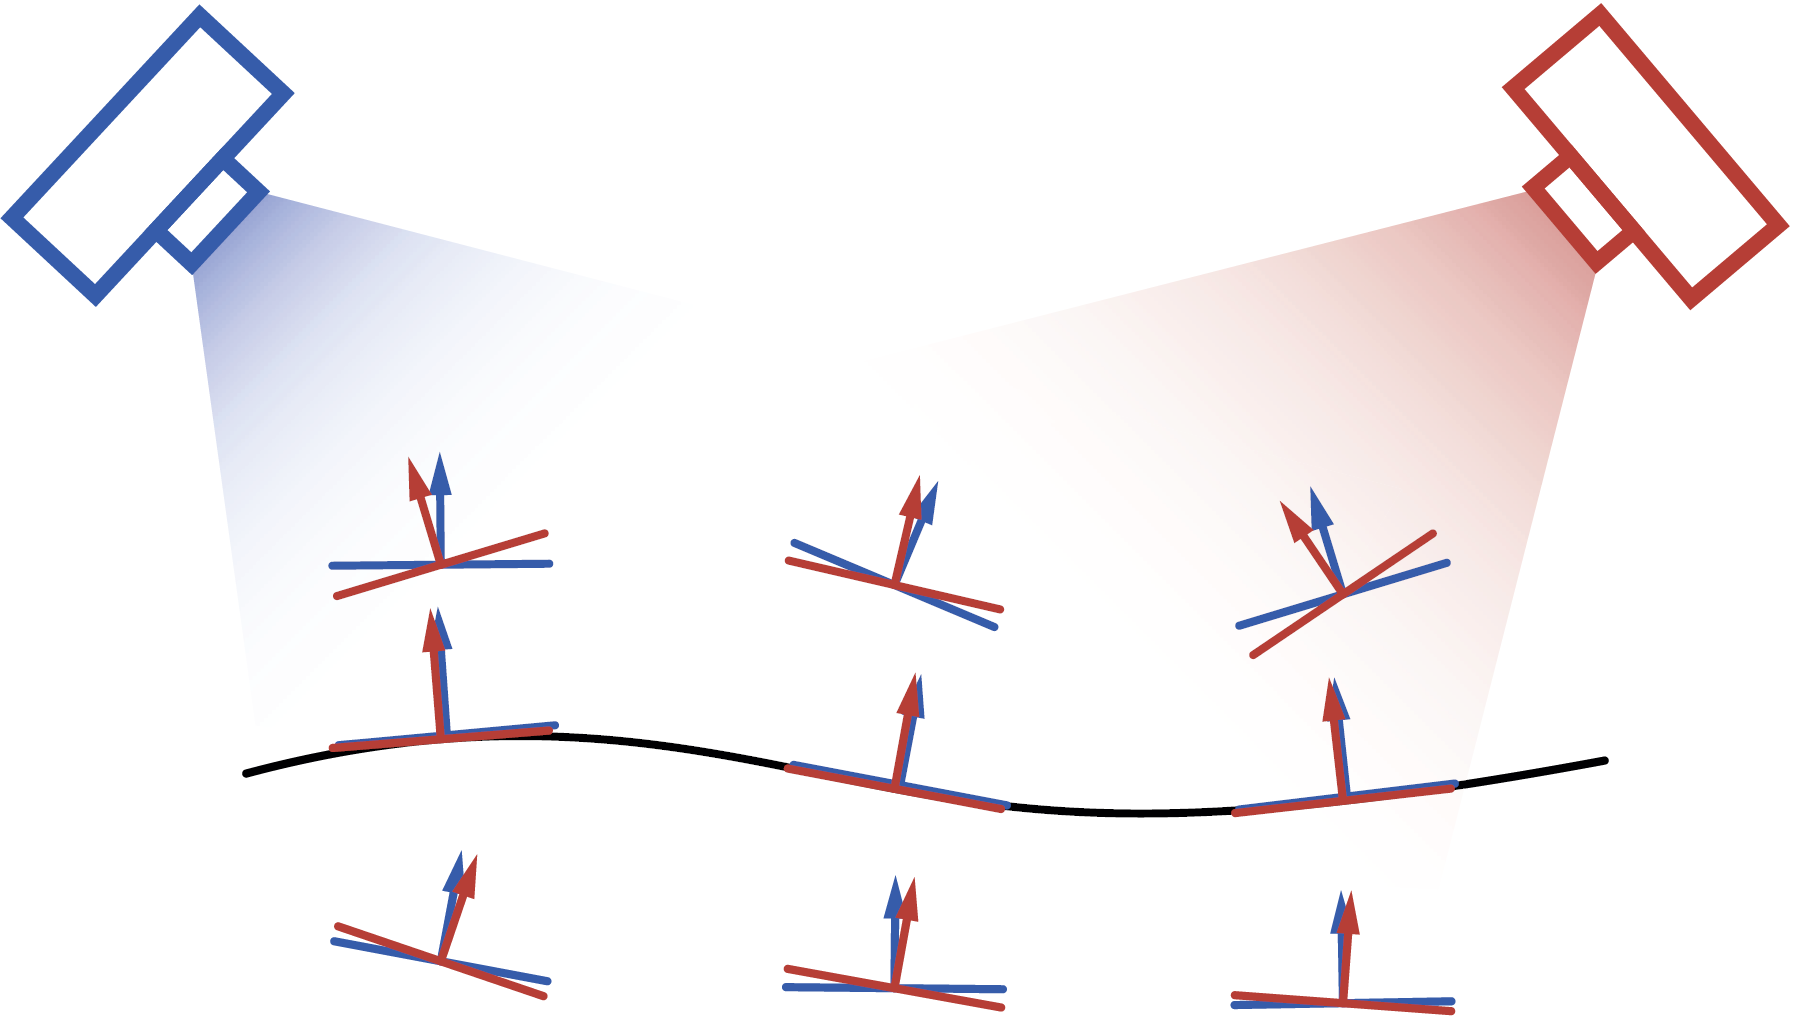
\includegraphics[width=0.5\textwidth]{02_grundlagenDerDeflektometrie/rekonstruktion/rekonstruktionUndRegularisierungsproblem/figures/stereoVerfahren}
	\caption[Stereo-Methode zur Lösung des Regularisierungsproblems]{Stereo-Methode zur Auflösung der Mehrdeutigkeit der Normalenfelder. Die eingezeichneten Pfeile sind die potentiellen Normalenvektoren auf unterschiedlichen Höhen. \cite{stereoDeflektometrie}}
	\label{img:stereoVerfahren}
\end{figure}
%
\noindent
Schließlich ist es möglich, aus dem Normalenfeld die räumlichen Informationen der Oberfläche zu berechnen.
Dafür kann man zunächst aus den Normalenvektoren die zugehörigen Tangentialebenen berechnen, die über je zwei Richtungsvektoren definiert sind.
Diese Richtungsvektoren bilden die Tangentialfelder des Prüfobjekts.
Man kann über eine Integration der Tangentialfelder in ausgewählte Richtungen Kurven bestimmen, die auf der Oberfläche des Objekts liegen.
Durch diese Integration erhält man einen Höhenzusammen\-hang der Oberflächenpunkte.
Wenn zusätzlich die Lage eines Oberflächenpunkts im Raum gegeben ist, kann man die Positionen der Oberflächenpunkte im Raum angeben \cite{kit_werling}.
}
%

}

%Qualitative Sichtprüfung
{
	\FloatBarrier
    \section{Qualitative Sichtprüfung}
    \label{sec:qualitativeSichtpruefung}
    Der Bereich der qualitativen Sichtprüfung hat grundlegend die Aufgabe, spiegelnde Oberflächen nach bestimmten Kriterien in gut und fehlerhaft zu unterteilen.
Die Aufbauten für solche Verfahren sehen in der Regel ähnlich aus wie auch in Abbildung \ref{img:aufbau}.
Zur Analyse dieser spiegelnden Oberflächen ist es nicht unbedingt nötig, zuerst ein dreidimensionales Oberflächenmodell zu erzeugen.
Ein wesentlicher Unterschied ist deshalb, dass die Informationen über den Systemaufbau nicht zwingend notwendig für Berechnungen sind.
Um eine möglichst allgemein einsetzbare Lösung zu entwickeln, ist dies ein essenzieller Vorteil.
Die Vorgehensweise bei diesen Verfahren basiert in den meisten Fällen darauf, die Abweichungen der Oberflächenstruktur zu einem Referenzobjekt zu bewerten.
Abhängig von den einzelnen Oberflächenmerkmalen können verschiedene Muster und Strategien zur Auswertung eingesetzt werden.

\p
In seiner Dissertation \glqq Deflektometrie zur automatischen Sichtprüfung und Rekonstruktion spiegelnder Oberflächen\grqq ~\cite{kit_werling} listet Stefan Bruno Werling vom Karlsruher Institut für Technologie einige Auswertungsmöglichkeiten auf.
Daraus sind die Folgenden eine Auswahl seiner Strategien:

\begin{itemize}
	\item Untersucht man auf der Oberfläche eines Objekts ein sinusoidales Streifenmuster, dann können im Frequenzraum Abweichungen des Musters von einem \glqq Idealmuster\grqq ~bzw. Referenzmuster festgestellt werden.
	Dadurch entdeckt man Unterschiede in der Oberflächenkrüm\-mung.
	Die Transformation des Bildes in den Frequenzraum wird durch die Fourier-Transformation erreicht.
	
	\item Nutzt man zur Auswertung ein Schachbrettmuster, so können durch die Wahl eines geeigneten Schwellwerts bestimmte Flächen segmentiert und geometrisch analysiert werden.
	Nach der Analyse sollen Anomalien der geometrischen Merkmale Aussagen über die Krümmung treffen.
	
	\item Besonders kleine Fehler und Defekte der Oberflächenstruktur lassen sich an Hell-Dunkelübergängen gut hervorheben.
	Hierfür kann man einfache Streifenmuster analysieren, wie es in Abbildung \ref{img:scratch} gezeigt ist.
	Dieses Verfahren wird im Kapitel \ref{chp:sichtpruefungDurchLichtstreuung} näher beschrieben.
\end{itemize}

\begin{figure}[H]
	\centering
	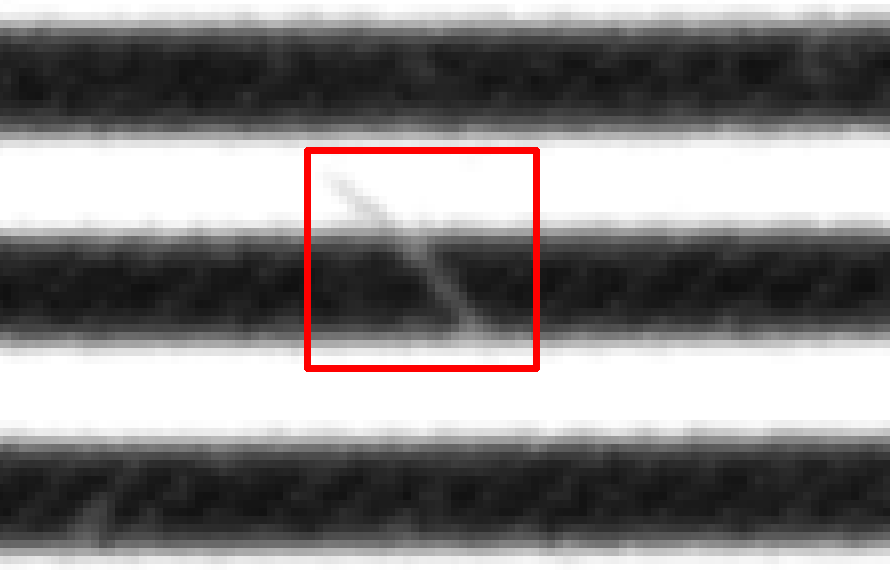
\includegraphics[width=0.5\textwidth]{02_grundlagenDerDeflektometrie/qualitativeSichtpruefung/figures/scratch}
	\caption[Kratzer an Hell-Dunkel-Übergang eines Streifenmusters]{Kratzer an Hell-Dunkel-Übergang eines Streifenmusters}
	\label{img:scratch}
\end{figure}

\noindent
Neben diesen Verfahren gibt es auch noch die Möglichkeit, die Krümmung zu analysieren, indem man die Zuordnung zwischen Kamera- und Bildschirmkoordinaten (siehe Abschnitt \ref{sec:rekonstruktion}) auswertet.
Analytisch betrachtet ändert sich bei starken lokalen Krümmungen der Oberfläche auch die Oberflächennormale an der lokalen Stelle besonders stark.
Mit dem Reflexionsgesetz wird damit kenntlich, dass lokal in der Reflexion große Abweichungen von einer ebenen Spiegelung auftreten.
Die Abweichung von einer ebenen Spiegelung lässt sich in der beschriebenen Zuordnung direkt erkennen, ohne weitere Systemparameter berücksichtigen zu müssen.
Dies wird im Abschnitt \ref{sec:auswertungDeflektometrischeRegistrierung} genauer behandelt.

\p
Durch die Variabilität der deflektometrische Verfahren und der vielen Möglichkeiten der qualitativen Sichtprüfung lassen sich z. B. durch Veränderung bestimmter Muster zahlreiche verschiedene Verfahren aufstellen, um eine Objektoberfläche zu analysieren.
Aus dem Grund wird keine allgemeine Funktionsweise von deflektometrischen Verfahren für die qualitative Sichtprüfung beschrieben, sondern auf konkrete Verfahren eingegangen, wie es z. B. in Kapitel \ref{chp:sichtpruefungDurchLichtstreuung} ausgeführt wird.
}